% lintrans - The linear transformation visualizer
% Copyright (C) 2021-2022 D. Dyson (DoctorDalek1963)

% This program is licensed under GNU GPLv3, available here:
% <https://www.gnu.org/licenses/gpl-3.0.html>

\documentclass[../development.tex]{subfiles}

\begin{document}

\subsubsection{The first version numbers\label{development:fumbling-with-semver:the-first-version-numbers}}

At this point, I've been developing lintrans for quite a while, but I don't have any kind of version numbers yet. I wanted to fix this, to keep track of versions through history. SemVer\cite{semver-2.0.0} is a system of numbering versions of software that ensures compatibility across versions and gives semantic meaning to the version numbers.

My first foray into using SemVer was to declare \texttt{lintrans} at this point to be \texttt{0.1.0-alpha}. In retrospect, these early versions don't make much sense. I didn't release anything for anyone else to use until version \texttt{0.3.0}, so everything before then doesn't make much sense and should probably just be ignored.

I then made a few adjustments to syntax and documentation before declaring version \texttt{0.1.1-alpha} just over 24 hours later. This one was completely unnecessary in hindsight and I think I was just excited about being able to tag git commits. Additionally, there is a \pyinline{__version__} variable in the root of the package, and the value of this variable is still \pyinline{"0.1.0-alpha"} at the \texttt{v0.1.1-alpha} tag because I forgot to update it before I tagged the commit, and I didn't know how to fix it at the time.

\subsubsection{Licensing\label{development:fumbling-with-semver:licensing}}

Using version numbers reminded me of licensing. I was already using the GNU GPLv3\cite{gnu-gplv3} for \texttt{lintrans} and most of my other projects, so I just wanted to add the copyright notice to all the source files of the project, as per the license. I already had the \texttt{COPYING} file in the project root with the full license, as required.

The notice looks like this\footnote{I'm calling myself D. Dyson here because my name is Dyson, and I was in the process of getting it legally changed to Dyson Dyson when I made this change. I can't attribute this copyright to Dyson, since that's already a registered trademark of Dyson Limited. Calling myself Dyson Dyson felt strange, especially since it wasn't even my legal name at the time. So I chose to use D. Dyson instead.}:

\begin{minted}{python}
# lintrans - The linear transformation visualizer
# Copyright (C) 2021-2022 D. Dyson (DoctorDalek1963)

# This program is licensed under GNU GPLv3, available here:
# <https://www.gnu.org/licenses/gpl-3.0.html>
\end{minted}

\subsubsection{Making the package executable\label{development:fumbling-with-semver:making-the-package-executable}}

So far, I'd been running the program by running a separate script called \texttt{run\_gui.py}, but Python lets you make a package executable by creating a file called \texttt{\_\_main\_\_.py} in the project root. You can then run it by using the command \mintinline{sh}{python -m package_name}. This will make the whole program more cohesive by integrating the execution into the same directory as the source library code. I just moved the script here and changed its docstring a little bit.

%: 847cdf61f64b30e81edf0821b7a8d2eb060fb825
%: src/lintrans/__main__.py:9-19

Somehow this caused a conflict between my \pyinline{lintrans.typing} package, which contained custom types like \pyinline{MatrixType}, and the standard library \pyinline{typing} package, so I had to rename mine to \pyinline{lintrans.typing_}.

\subsubsection{Improving the documentation\label{development:fumbling-with-semver:improving-the-documentation}}

Throughout the whole project, I've been using GitHub Actions\cite{github-actions-docs} to automatically do things like test and lint my code, as well as compile the documentation whenever I push my changes to GitHub. I recently learned about \texttt{pylint}'s ability to generate a graph of all the internal imports in a package\cite{pylint-2.12.2-graph-docs}. I decided to generate this graph automatically and add it to my documentation.

%: 39a3727fca69ea65571a15c55741578abce1e763
%: .github/workflows/compile-docs.yaml language=yaml

\begin{figure}[H]
	\centering
	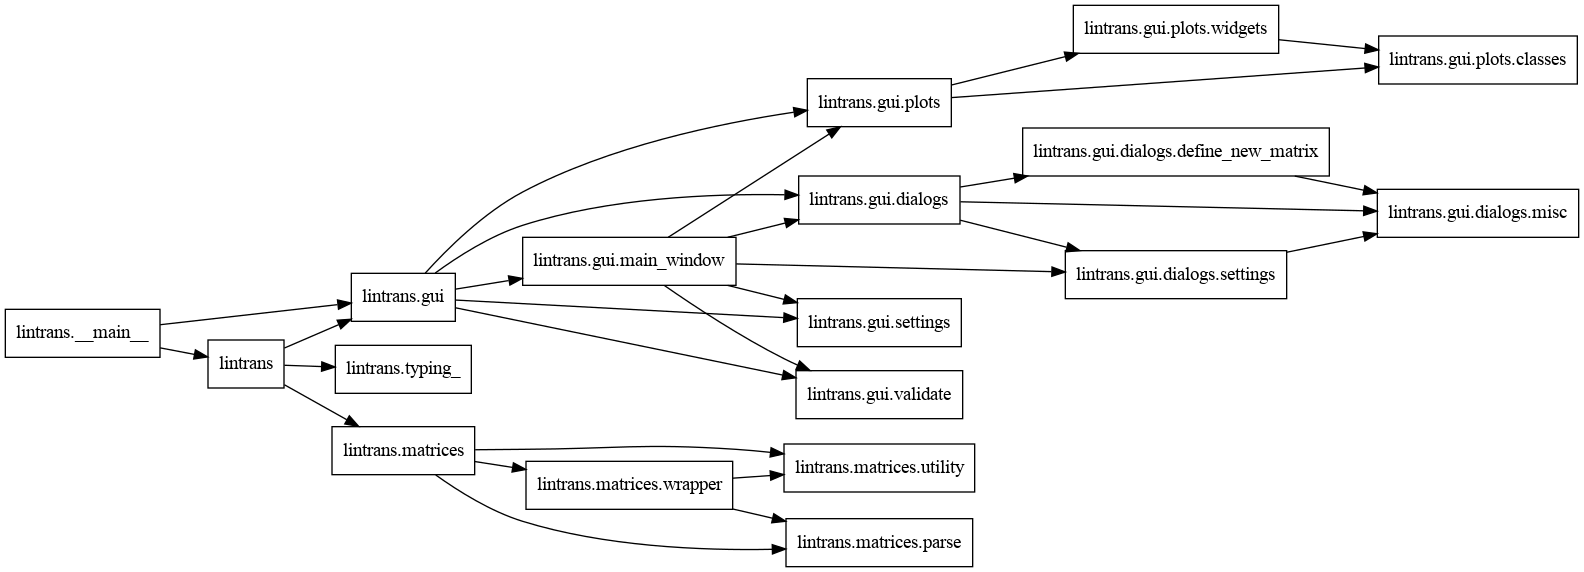
\includegraphics[width=\linewidth]{development/39a3727fca69ea65571a15c55741578abce1e763/int-imports.png}
	\caption{The internal imports graph}
	\label{fig:development:39a3727fca69ea65571a15c55741578abce1e763:int-imports.png}
\end{figure}

\subsubsection{Fixing the colours\label{development:fumbling-with-semver:fixing-the-colours}}

Now that I was using version numbers, I thought it was finally time to fix the colours in accordance with \S\ref{design:usability-features}. I decided to use red and blue for the basis vectors, since these are the most easily distinguished colours for colour blind users. I decided to keep the green colour and use it for the eigenvectors and eigenlines. These are very visually distinct from the basis vectors, so I don't think I need to further distinguish them with colours. Red-green colour blind users should be able to tell them apart with ease.

\begin{figure}[H]
	\centering
	\includegraphics[width=0.85\linewidth]{development/39a3727fca69ea65571a15c55741578abce1e763/gui.png}
	\caption{The old colours}
	\label{fig:development:39a3727fca69ea65571a15c55741578abce1e763:gui.png}
\end{figure}

\begin{figure}[H]
	\centering
	\includegraphics[width=0.85\linewidth]{development/be37c68dd38d64ac82a7d23c7801c5ca8a0da518/gui.png}
	\caption{The new colours}
	\label{fig:development:be37c68dd38d64ac82a7d23c7801c5ca8a0da518:gui.png}
\end{figure}

\subsubsection{Compiling for release\label{development:fumbling-with-semver:compiling-for-release}}

At this point, I felt ready to show \texttt{lintrans} to some teachers. Obviously I didn't expect them to have a modern version of Python to run the program, especially not on a school laptop, so I had to compile the program. I had a look at things like Nuitka\cite{nuitka-docs}, but I had a few issues with it and it took ages to compile. Eventually I chose PyInstaller\cite{pyinstaller-4.10-docs}, which I've used to compile Python programs before. It's fast and effective and works very well.

I use Ubuntu as my daily driver, so I don't really want to spin up a Windows virtual machine and following some exact steps every time I want to compile \texttt{lintrans} for release, so I automated the process with GitHub Actions.

%: 9d0cbe69c596c04a07809a288d72b5e624f485d7
%: .github/workflows/compile-release.yaml language=yaml

This workflow only runs when I push a tag containing a version number. It firstly installs Python\footnote{There's a mistake on line 14. There is no strategy matrix, so \enquote{\texttt{\$\{\{ matrix.python-version \}\}}} is treated as plain text rather than an actual version number. This was caused by copying a previous workflow. The actual version that it installs is fine, though. It's only the name of the step that doesn't look right.} and then lints and tests everything. If that all passes, then it compiles \texttt{lintrans} on Ubuntu, macOS, and Windows. Then it publishes the compiled binaries to a GitHub draft release. I then go in when it's finished to add a description to the release and publish it.

Now that I had this in place, I released version \texttt{v0.2.0-alpha}.

After some minor adjustments, such as including the tag name in the binary name, and installing UPX\cite{upx-github} for the Linux compilation\footnote{UPX is designed to compress executable files, but I later learned that PyInstaller doesn't even use UPX on Linux; it only uses it on Windows.}, I released \texttt{v0.2.0} just 6 hours later.

I made a few minor adjustments to the workflows, but soon moved on from this version number fiasco and started doing more actual work.

\end{document}
